%!TEX TS-program = pdflatex

% Copyright (c) 2015, 2016 Mario Mlačak, mmlacak@gmail.com
% Licensed and published as Public Domain work.
% https://en.wikipedia.org/wiki/Public_domain

\documentclass[a5paper,12pt,draft]{book} % draft = DEBUG

\usepackage[utf8]{inputenc}
% \usepackage[T1]{fontenc}

\usepackage{charter}
\renewcommand{\rmdefault}{bch}

\usepackage{helvet}
\renewcommand{\sfdefault}{phv}

\renewcommand{\ttdefault}{pcr}

% \renewcommand{\familydefault}{\sfdefault} % \rmdefault

% left = inner, right = outer
\usepackage[top=15.0mm, bottom=20.0mm, left=15.0mm, right=20.0mm]{geometry}
\setlength{\marginparwidth}{0.0pt}
\setlength{\footskip}{20.0pt}

% \usepackage{showframe} % DEBUG

\usepackage[final]{graphicx} % demo = DEBUG
\graphicspath{ {../draft/} }
% \graphicspath{ {../gfx/} }
\usepackage{wrapfig}

\usepackage{hyperref}
\hypersetup{final=true, unicode=true, colorlinks=true}
\hypersetup{pdftitle={Croatian chess and other variants},
            pdfauthor={Mario Mlačak},
            pdfsubject={Chess variants},
            pdfkeywords={chess, variants}}
% \urlstyle{same}

\pagestyle {plain}
\setlength{\parindent}{1.5em}
\setlength{\parskip}{1.0em}
\emergencystretch=1.5em % 1.5em = half of what \sloppy would use


% Book ----------------------------------------------------------------
\begin{document}

% Title page ----------------------------------------------------------
\begin{titlepage}
\vspace*{\stretch{2}}
\begin{center}
    \textbf{\huge{Croatian chess}} \\
    \large{and other variants} \\ [2.0cm]

    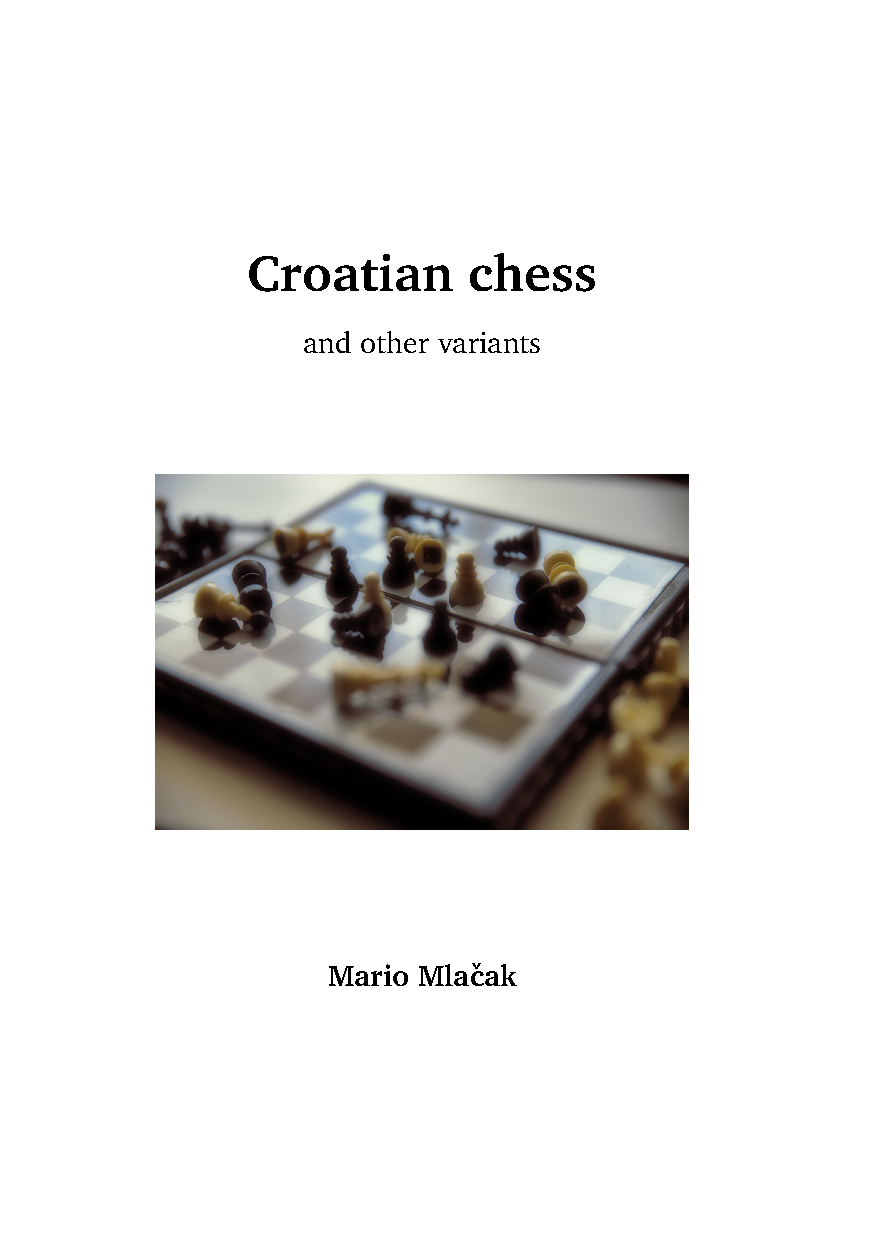
\includegraphics[width=0.9\textwidth, keepaspectratio=true]{crochess.jpg} \\ [2.0cm]

    \textbf{\large{Mario Mlačak}} \\ [2.0cm]
\end{center}
\vspace{\stretch{1}}
\end{titlepage}
% ---------------------------------------------------------- Title page

% Empty page ----------------------------------------------------------
\thispagestyle{empty}
\vspace*{0.1\textheight}
\clearpage
% ---------------------------------------------------------- Empty page

% Dedication page -----------------------------------------------------
\thispagestyle{empty}
\vspace*{0.2\textheight}
\hfill{Dedicated to Miranda.}
\clearpage
% ----------------------------------------------------- Dedication page

% Publisher page ------------------------------------------------------
\thispagestyle{empty}
\vspace*{0.1\textheight}
\begin{center}
    \emph{Mario Mlačak} \\
    \textbf{Croatian chess} \\
    and other variants \\ [2.0em]

    \emph{Copyright} \\
    Copyright \copyright \hspace{0.2ex} 2009 -- 2016 Mario Mlačak \\
    \href{mailto:mmlacak@gmail.com}{mmlacak@gmail.com} \\ [2.0em]

    \emph{Legal} \\
    This book is published as Public Domain work. \\
    \href{https://en.wikipedia.org/wiki/Public\_domain}{https://en.wikipedia.org/wiki/Public\_domain} \\ [2.0em]

    \emph{Third, revised edition} \\
    \today \\
    Zagreb

    \vfill

    \LaTeXe
    \vspace{0.1\textheight}
\end{center}
\clearpage
% ------------------------------------------------------ Publisher page

% Inner title page ----------------------------------------------------
\thispagestyle{empty}
\vspace*{0.2\textheight}
\begin{center}
    \textbf{\Large{Croatian chess}} \\ [1.0em]
    \large{and other variants} \\ [1.0em]
    \small{3rd, revised edition} \\ [2.0cm]
    \vspace*{0.2\textheight}

    \textbf{\large{Mario Mlačak}} \\ [1.0em]
    \small{\today} % \\ [2.0cm]
\end{center}
\clearpage
% ---------------------------------------------------- Inner title page

% Empty page ----------------------------------------------------------
\thispagestyle{empty}
\vspace*{0.1\textheight}
\clearpage
% ---------------------------------------------------------- Empty page

% Gratitude page ------------------------------------------------------
\thispagestyle{empty}
\vspace*{0.2\textheight}
\begin{flushright}
My most sincere gratitude to:

Valentina Štefanić \\
Kristina Mlačak \\
Slavko Štefanić

and many, many others.

Thank you all.
\end{flushright}
\clearpage
% ------------------------------------------------------ Gratitude page

% Empty page ----------------------------------------------------------
\thispagestyle{empty}
\vspace*{0.1\textheight}
\clearpage
% ---------------------------------------------------------- Empty page

% Introduction chapter ------------------------------------------------
\chapter*{Introduction}
\addcontentsline{toc}{chapter}{Introduction}

\begin{flushright}
\parbox{0.6\textwidth}{
\emph{Life's too short for chess. \\
\hspace*{\fill}{\textperiodcentered \textperiodcentered \textperiodcentered \hspace*{0.2em} Henry James Byron} } }
\end{flushright}

\noindent
I was in my aunt's house, on the border of a small village.
Through window walled garden and small brook was visible just
behind the house. And hills in the distance. Early afternoon Sun
was casting its orange rays into warm room. It was cold outside.

My cousin approached me with some nifty gizmo. He was a
few years older then me and was already going to school. \\
"Here, look at what I got." \\
"What's that?" \\
"Chess set. Wanna try? Lemme show you." \\
"Sure."

It was small plasticky, fiddly thing designed to fit into winter's
coat pocket, to be used on the go. Folding board was also used to
hold all pieces in it. Each piece was as small as humanely usable.
Each field had a hole in the middle. Bellow each piece there was
small rod fitting into those holes. It was colored all in red and ivory.

Short lesson revealed it's not that difficult to grasp what's going
on. Within minutes I picked it up. First match was, predictably, a
complete disaster. On the second go my cousin forgot about a piece,
and I grabbed his Queen gleefully. He surrendered.

After he left me with a new widget, I was intrigued. I wasn't
about playing the game, though. I was more into redesign it. Could it
be made better, more challenging, or just different? \\
'Why not make Knight jump longer, say 3 by 1 fields?' \\
'Hmmmm...' \\
'Nah, that would make jump too long for such a small board.'

Outside, the Sun was shining red.
\clearpage
% ------------------------------------------------ Introduction chapter

% Prerequisites chapter -----------------------------------------------
\chapter*{Prerequisites}
\addcontentsline{toc}{chapter}{Prerequisites}

\begin{flushright}
\parbox{0.7\textwidth}{
\emph{It does not matter how slowly you go as long as you do not stop. \\
\hspace*{\fill}{\textperiodcentered \textperiodcentered \textperiodcentered \hspace*{0.2em} Confucius} } }
\end{flushright}

\noindent
This document describes new variants of chess, new pieces
and rules. In this document I'll describe only even variants, since
generating odd ones from there is an exercise in simplicity. Please,
see 'Even variant', 'Odd variant' in the Definitions bellow.

\textbf{\huge{TODO :: FIX ME !!!}} % TODO :: FIX ME !!!

In this document I'm assuming you have the complete prior
knowledge of classical chess pieces and rules. If not, please visit
Wikipedia entry on this subject at \\
\href{https://en.wikipedia.org/wiki/Rules\_of\_chess}{https://en.wikipedia.org/wiki/Rules\_of\_chess}.
\clearpage
% ----------------------------------------------- Prerequisites chapter

% Classical Game chapter ----------------------------------------------
\chapter*{Classical Game}
\addcontentsline{toc}{chapter}{Classical Game}

\begin{flushright}
\parbox{0.8\textwidth}{
\emph{A great war leaves the country with three armies -
an army of cripples, an army of mourners, and an army of thieves. \\
\hspace*{\fill}{\textperiodcentered \textperiodcentered \textperiodcentered \hspace*{0.2em} German proverb} } }
\end{flushright}

\noindent
About classical chess is written really everything already, and I
have nothing to add. Except for illustration of initial setup, so that
you can accustom yourself with rendition of pieces used in this text.

Note that in Odd Classical Game, since it's played on 7 x 7 board,
there is no en-passant move. This is so because of very small board
there is no room for a Pawn to perform 2-field initial move without,
at the same time, preventing opponent to do the same at the same file.

\noindent
\begin{figure}[t]
\includegraphics[width=1.0\textwidth, keepaspectratio=true]{boards/02_classical.png}
\caption{Classical board}
\label{fig:classical_chess}
% \centering
\end{figure}

\clearpage
% ---------------------------------------------- Classical Game chapter

% Croatian Ties chapter -----------------------------------------------
\chapter*{Croatian Ties}
\addcontentsline{toc}{chapter}{Croatian Ties}

\begin{flushright}
\parbox{0.7\textwidth}{
\emph{Secrecy is the first essential in affairs of the State. \\
\hspace*{\fill}{\textperiodcentered \textperiodcentered \textperiodcentered \hspace*{0.2em} De Richelieu} } }
\end{flushright}

\noindent
Croatian Ties is chess variant which is played on 10 x 10 board,
with silver and red fields and dark silver and dark red pieces.
In algebraic notation, columns are enumerated from 'a' to 'j',
and rows are enumerated from '1' to '10'. A new piece is
introduced, Pegasus.

\clearpage

\section*{Pegasus}
\addcontentsline{toc}{section}{Pegasus}

\noindent
\begin{wrapfigure}[9]{l}{0.4\textwidth}
\includegraphics[width=0.4\textwidth, keepaspectratio=true]{pieces/07_pegasus.png}
\caption{Pegasus}
\label{fig:pegasus}
% % \centering
\end{wrapfigure}
Pegasus moves similarly to Knight, but it can continue its jumpy movement
until another piece is encountered, or it runs out of board. Note that once
in movement, Pegasus can not change its' heading.

Pegasus symbol in algebraic notation is 'G', to avoid confusion with Pawn.

\vspace{2\baselineskip}

\noindent
\begin{wrapfigure}[12]{l}{0.5\textwidth}
\includegraphics[width=0.5\textwidth, keepaspectratio=true]{examples/01_move_pegasus_initial.png}
\caption{Pegasus initial step}
\label{fig:pegasus_initial_step}
% % \centering
\end{wrapfigure}
In the example on the left we have Pegasus with all valid initial move directions
marked. These all are the same as valid moves for Knight. Pegasus' movement is not
hampered by surrounding piece, if it's placed on any unmarked field. Pegasus can
"jump" over it just as Knight would.

\clearpage

\noindent
% \begin{figure}[t]
\begin{figure}[!t]
\includegraphics[width=1.0\textwidth, keepaspectratio=true]{examples/02_move_pegasus_direction.png}
\caption{Pegasus move direction}
\label{fig:pegasus_move_direction}
% \centering
\end{figure}
Once direction is chosen Pegasus can continue its' movement performing one jump
after another in order from nearest field to furthest. Here, this is marked
with green arrows. Accessible fields are marked 1 to 4, in order of accessibility,
from nearest to furthest. Again, once direction is chosen it can't be changed
anymore. For instance, after reaching field 2 it's not allowed to change
direction to 2f (or any other greyed-out arrow).

\clearpage

\noindent
% \begin{figure}[t]
\begin{figure}[!t]
\includegraphics[width=1.0\textwidth, keepaspectratio=true]{examples/03_move_pegasus.png}
\caption{Pegasus moves}
\label{fig:pegasus_moves}
% \centering
\end{figure}
Move along arrow is called step. Field at which arrow points to is called step field.
Pegasus can "jump" over pieces on non-step fields, Rooks in example above. Numbers
here enumerate directions of movement. Own piece on step field stops Pegasus at
preceding step field, see direction 2. Opponent's piece on step field can be captured.
Just as with any other piece that would finish the move, meaning Pegasus would have to
stop at captured step field, see direction 1.

\clearpage

\section*{En passant}
\addcontentsline{toc}{section}{En passant}

\noindent
\begin{wrapfigure}{l}{0.4\textwidth}
\includegraphics[width=0.4\textwidth, keepaspectratio=true]{en_passants/04_croatian_ties_en_passant.png}
\caption{En passant}
\label{fig:cc_en_passant}
% % \centering
\end{wrapfigure}
En passant is identical to one in Classic Chess, only difference is that Pawn can now
move longer on initial turn, up to 3 fields in this instance. As expected, all passed-by
opponent's Pawns also gain en passant opportunity.

Passed-by opponents are those which are at most at the same row in which Pawn has ended its'
initial move, or which are closer to Pawn's initial position.

In example on left, if light Pawn's initial move was 3 fields long, ending in field marked 2,
both dark Pawns would have en passant opportunity. Naturaly, if initial move was only 2 fields
long, ending in field marked 1, only dark Pawn on the right would gain en passant opportunity.

\clearpage

\section*{Castling}
\addcontentsline{toc}{section}{Castling}

Castling is essentially the same as it is in Classical Chess, only real difference is that
King can move either 2 or 3 fields across. All other constraints from Classical Chess still
applies, described in detail here \\
\href{https://en.wikipedia.org/wiki/Castling}{https://en.wikipedia.org/wiki/Castling}.

\noindent
\begin{figure}[!h]
% \begin{figure}[!t]
\includegraphics[width=1.0\textwidth, keepaspectratio=true]{castlings/04_croatian_ties_castling.png}
\caption{Castling}
\label{fig:cc_castling}
% \centering
\end{figure}

In example above, all valid King's castling moves are numbered. Regardless if King performs
long or short castling move, Rook would always end up on field next to King, on opposite side
of it, i.e. closer to center.

\noindent
\begin{figure}[!h]
% \begin{figure}[!t]
\includegraphics[width=1.0\textwidth, keepaspectratio=true]{castlings/long_left/04_croatian_ties_castling_long_left.png}
\caption{Castling long left}
\label{fig:cc_castling_long_left}
% \centering
\end{figure}

In this example King was castling long to the left. Initial King's position is marked with "K".
After castling is finished, left Rook ends up at field immediately on the right to the King.

\clearpage

\section*{Initial setup}
\addcontentsline{toc}{section}{Initial setup}

Initial setup for Light player is (mirrored for Dark one):
\texttt{PPPPPPPPPP \\
        RGNBQKBNGR}, \\
or more conveniently, as seen in this image:

\noindent
% \begin{figure}[t]
\begin{figure}[h]
\includegraphics[width=1.0\textwidth, keepaspectratio=true]{boards/04_croatian_ties.png}
\caption{Croatian Ties board}
\label{fig:croatian_ties}
% \centering
\end{figure}

\clearpage
% ----------------------------------------------- Croatian Ties chapter

% Mayan Ascendancy chapter --------------------------------------------
\chapter*{Mayan Ascendancy}
\addcontentsline{toc}{chapter}{Mayan Ascendancy}

\begin{flushright}
\parbox{0.8\textwidth}{
\emph{The world has achieved brilliance without wisdom, power without
conscience. Our is a world of nuclear giants and ethical infants. \\
\hspace*{\fill}{\textperiodcentered \textperiodcentered \textperiodcentered \hspace*{0.2em} Omar Nelson Bradley} } }
\end{flushright}

\noindent
Mayan Ascendancy is chess variant which is played on 12 x 12 board with
yellow and blue fields and with dark yellow and dark blue pieces. In
algebraic notation, columns are enumerated from 'a' to 'l', and rows are
enumerated from '1' to '12'. A new piece is introduced, Pyramid.

\clearpage

\section*{Pyramid}
\addcontentsline{toc}{section}{Pyramid}

\noindent
\begin{wrapfigure}[12]{l}{0.4\textwidth}
\includegraphics[width=0.4\textwidth, keepaspectratio=true]{pieces/08_pyramid.png}
\caption{Pyramid}
\label{fig:pyramid}
% % \centering
\end{wrapfigure}
Pyramid is passive piece, meaning it can't move on its' own, it has to be
activated first. This is done by capturing a field at which Pyramid stands
with your own other piece, for instance Bishop, and then Pyramid can move
further.

Once activated Pyramid moves similar to Rook, only real difference is that
it can move for only so many fields as piece activating it has moved.

Pyramid can't check opponent's King, and consequently can't contribute to
checkmate.

In algebraic notation symbol for Pyramid is 'A', to avoid confusion with Pawn.

\subsection*{Momentum}
\addcontentsline{toc}{subsection}{Momentum}

% TODO

\clearpage

\subsection*{Promotion}
\addcontentsline{toc}{subsection}{Promotion}

Pyramid can promote own Pawns, but only on opponent's side of the board.
Promotion is done by activating Pyramid which then marks Pawn for promotion
by touching either Pawn or field at which it stands. Pyramid then leaves
board as if it was captured, and Pawn is replaced by desired piece, for
instance Queen.

Both Pyramid and Pawn in question has to reside on opponent's side of the
board before promotion can take place. Piece which activates Pyramid need
not to be on opponent's side of the board.

Piece which Pawn can be promoted to is from the set of all starting pieces,
except King. This promoting-to piece is not limited to pieces already being
captured.

\clearpage

\noindent
\begin{figure}[!h]
% \begin{figure}[!t]
\includegraphics[width=1.0\textwidth, keepaspectratio=true]{examples/04_move_pyramid_promo_init.png}
\caption{Promotion start}
\label{fig:ma_promo_init}
% \centering
\end{figure}

Here, note only step fields are counted as traveled over by Pegasus. This
count is called momentum. After activation Pyramid would be limited to move
at most 4 fields across, i.e. at most the momentum it received from activating
piece.

\clearpage

\noindent
\begin{figure}[!h]
% \begin{figure}[!t]
\includegraphics[width=1.0\textwidth, keepaspectratio=true]{examples/05_move_pyramid_promo_activate.png}
\caption{Promotion, Pyramid activated}
\label{fig:ma_promo_activate}
% \centering
\end{figure}

Above, Pegasus captured field at which Pyramid was situated, arrows now show
all possible moves by Pyramid. Only full move to the right leads to promotion,
shown in red. Just as Rook, Pyramid can't advance past Pawn.

\clearpage

\noindent
\begin{figure}[!h]
% \begin{figure}[!t]
\includegraphics[width=1.0\textwidth, keepaspectratio=true]{examples/06_move_pyramid_promo_end.png}
\caption{Promotion end}
\label{fig:ma_promo_end}
% \centering
\end{figure}

Now that Pyramid has reached Pawn, it is removed from the board and piece of
choice, in this instance Queen, replaces Pawn.

\clearpage

\subsection*{Conversion}
\addcontentsline{toc}{subsection}{Conversion}

Pyramid can convert opponent's pieces, except King, but only on own side of
the board. Conversion is done by activating Pyramid which then marks opponent's
piece for conversion by touching either piece or field at which it stands. Now
Pyramid leaves the board as if it was captured, and opponent's piece is replaced
by own piece of the same type.

Both Pyramid and opponent's piece has to reside on own side of the board
before conversion can take place. Piece which activates Pyramid need not
to be on own side of the board. As with promotion, conversion is not limited
to pieces which has been captured.

Note that Pyramid might just as well capture opponent's piece. Differences are
who leaves chess board, and what remains on captured field. Capture itself with
Pyramid is in no way different than that with Rook, provided that Pyramid can
reach opponent's piece, i.e. that it get enough momentum from activating piece.

\clearpage

\noindent
\begin{figure}[!h]
% \begin{figure}[!t]
\includegraphics[width=1.0\textwidth, keepaspectratio=true]{examples/07_move_pyramid_conversion_init.png}
\caption{Conversion start}
\label{fig:ma_conversion_init}
% \centering
\end{figure}

For classic pieces, step fields are just fields which piece traveled over,
in case of Bishop above that is 4 fields. Again, that is momentum Pyramid
will receive with activation and limits how far it could move afterwards.

\clearpage

\noindent
\begin{figure}[!h]
% \begin{figure}[!t]
\includegraphics[width=1.0\textwidth, keepaspectratio=true]{examples/08_move_pyramid_conversion_activated.png}
\caption{Conversion, Pyramid activated}
\label{fig:ma_conversion_activated}
% \centering
\end{figure}

Above, Bishop captured field at which Pyramid was situated, arrows now show
all possible moves by Pyramid. Only full move to the right leads to promotion,
shown in red. Again, just as Rook, Pyramid can't advance past opponent's Rook.

\clearpage

\noindent
\begin{figure}[!h]
% \begin{figure}[!t]
\includegraphics[width=1.0\textwidth, keepaspectratio=true]{examples/09_move_pyramid_conversion_end.png}
\caption{Conversion end}
\label{fig:ma_conversion_end}
% \centering
\end{figure}

Now that Pyramid has reached opponent's Rook, it is removed from the board and
own Rook replaces opponent's Rook. Capturing opponent's Rook would simply leave
Pyramid in place of it.

\clearpage

\subsection*{Cascading}
\addcontentsline{toc}{subsection}{Cascading}

% TODO

\clearpage

\section*{En passant}
\addcontentsline{toc}{section}{En passant}

\noindent
\begin{wrapfigure}{l}{0.4\textwidth}
\includegraphics[width=0.4\textwidth, keepaspectratio=true]{en_passants/06_mayan_ascendancy_en_passant.png}
\caption{En passant}
\label{fig:ma_en_passant}
% % \centering
\end{wrapfigure}
En passant is identical to one in Classic Chess, only difference is that Pawn can now
move longer on initial turn, up to 4 fields in this instance. As expected, all passed-by
opponent's Pawns also gain en passant opportunity.

In example on left, if light Pawn's initial move was 3 fields long, ending in field marked
2, two dark Pawns closest to light Pawn's initial position would have en passant opportunity,
in rows 1 and 2.

\clearpage

\section*{Castling}
\addcontentsline{toc}{section}{Castling}

Castling is essentially the same as it is in Classical Chess, only real difference is that
King can move 2, 3 or 4 fields across. All other constraints from Classical Chess still
applies.

\noindent
\begin{figure}[!h]
% \begin{figure}[!t]
\includegraphics[width=1.0\textwidth, keepaspectratio=true]{castlings/06_mayan_ascendancy_castling.png}
\caption{Castling}
\label{fig:ma_castling}
% \centering
\end{figure}

In example above, all valid King's castling moves are numbered. Regardless if King performs
long or short castling move, Rook would always end up on field next to King, on opposite side
of it, i.e. closer to center.

\noindent
\begin{figure}[!h]
% \begin{figure}[!t]
\includegraphics[width=1.0\textwidth, keepaspectratio=true]{castlings/long_left/06_mayan_ascendancy_castling_long_left.png}
\caption{Castling long left}
\label{fig:ma_castling_long_left}
% \centering
\end{figure}

In this example King was castling long to the left. Initial King's position is marked with "K".
After castling is finished, left Rook ends up at field immediately on the right to the King.

\clearpage

\section*{Initial setup}
\addcontentsline{toc}{section}{Initial setup}

Initial setup for Light player is (mirrored for Dark one):
\texttt{PPPPPPPPPPPP \\
        RGANBQKBNAGR}, \\
or more conveniently, as seen in this image:

\noindent
% \begin{figure}[t]
\begin{figure}[h]
\includegraphics[width=1.0\textwidth, keepaspectratio=true]{boards/06_mayan_ascendancy.png}
\caption{Mayan Ascendancy board}
\label{fig:mayan_ascendancy}
% \centering
\end{figure}

\clearpage
% -------------------------------------------- Mayan Ascendancy chapter

% Age of Aquarius chapter ---------------------------------------------
\chapter*{Age of Aquarius}
\addcontentsline{toc}{chapter}{Age of Aquarius}

\begin{flushright}
\parbox{0.8\textwidth}{
\emph{The greatest difficulty with the world is not its ability to produce, but the unwillingness to share. \\
\hspace*{\fill}{\textperiodcentered \textperiodcentered \textperiodcentered \hspace*{0.2em} Roy L. Smith} } }
\end{flushright}

\noindent
Age of Aquarius is chess variant which is played on 14 x 14 board,
with light yellow and light green fields and light tan-gold and
dark green pieces. In algebraic notation, columns are enumerated
from 'a' to 'n', and rows are enumerated from '1' to '14'. A new
piece is introduced, Unicorn.

\clearpage

\section*{Unicorn}
\addcontentsline{toc}{section}{Unicorn}

\noindent
\begin{wrapfigure}[5]{l}{0.4\textwidth}
\includegraphics[width=0.4\textwidth, keepaspectratio=true]{pieces/09_unicorn.png}
\caption{Unicorn}
\label{fig:unicorn}
% % \centering
\end{wrapfigure}
Unicorn is a piece similar to Knight, only it can jump longer on
opposite color fields. Just as Knight, Unicorn is not obstructed
by any piece in its' surroundings.

\vspace{8\baselineskip}

\noindent
\begin{wrapfigure}{l}{0.5\textwidth}
\includegraphics[width=0.5\textwidth, keepaspectratio=true]{examples/10_move_unicorn_same_color.png}
\caption{Unicorn short jump}
\label{fig:unicorn_short}
% % \centering
\end{wrapfigure}
On fields with the same color as Unicorn, it can move exactly the
same way Knight does.

\clearpage

\noindent
\begin{figure}[!h]
% \begin{figure}[!t]
\includegraphics[width=1.0\textwidth, keepaspectratio=true]{examples/11_move_unicorn_opposite_color.png}
\caption{Unicorn long jump}
\label{fig:unicorn_long}
% \centering
\end{figure}

On fields in opposite color to Unicorn's, Unicorn can jump much longer.
Again, just as Knight, Unicorn is not hampered by surrouding pieces.
Only own pieces on marked (i.e. step) fields can prevent Unicorn to move.
Opponent's pieces on step fields would, naturally, be captured.

\clearpage

\section*{En passant}
\addcontentsline{toc}{section}{En passant}

\noindent
\begin{wrapfigure}{l}{0.4\textwidth}
\includegraphics[width=0.4\textwidth, keepaspectratio=true]{en_passants/08_age_of_aquarius_en_passant.png}
\caption{En passant}
\label{fig:aoa_en_passant}
% % \centering
\end{wrapfigure}
En passant is identical to one in Classic Chess, only difference is that Pawn can now
move longer on initial turn, up to 5 fields in this instance. As expected, all passed-by
opponent's Pawns also gain en passant opportunity.

In example on left, if light Pawn's initial move was 4 fields long, ending in field marked
3, three dark Pawns closest to light Pawn's initial position would have en passant opportunity,
in rows 1, 2 and 3.

\clearpage

\section*{Castling}
\addcontentsline{toc}{section}{Castling}

Castling is essentially the same as it is in Classical Chess, only real difference is that
King can move 2, 3, 4 or 5 fields across. All other constraints from Classical Chess still
applies.

\noindent
\begin{figure}[!h]
% \begin{figure}[!t]
\includegraphics[width=1.0\textwidth, keepaspectratio=true]{castlings/08_age_of_aquarius_castling.png}
\caption{Castling}
\label{fig:aoa_castling}
% \centering
\end{figure}

In example above, all valid King's castling moves are numbered. Regardless if King performs
long or short castling move, Rook would always end up on field next to King, on opposite side
of it, i.e. closer to center.

\noindent
\begin{figure}[!h]
% \begin{figure}[!t]
\includegraphics[width=1.0\textwidth, keepaspectratio=true]{castlings/long_left/08_age_of_aquarius_castling_long_left.png}
\caption{Castling long left}
\label{fig:aoa_castling_long_left}
% \centering
\end{figure}

In this example King was castling long to the left. Initial King's position is marked with "K".
After castling is finished, left Rook ends up at field immediately on the right to the King.

\clearpage

\section*{Initial setup}
\addcontentsline{toc}{section}{Initial setup}

Initial setup for Light player is (mirrored for Dark one):
\texttt{PPPPPPPPPPPPPP \\
        RGAUNBQKBNUAGR}, \\
or more conveniently, as seen in this image:

\noindent
% \begin{figure}[t]
\begin{figure}[h]
\includegraphics[width=1.0\textwidth, keepaspectratio=true]{boards/08_age_of_aquarius.png}
\caption{Age of Aquarius board}
\label{fig:age_of_aquarius}
% \centering
\end{figure}

\clearpage
% --------------------------------------------- Age of Aquarius chapter

% Miranda's veil chapter ----------------------------------------------
\chapter*{Miranda's veil}
\addcontentsline{toc}{chapter}{Miranda's veil}

\begin{flushright}
\parbox{0.8\textwidth}{
\emph{Under all that we think, lives all we believe, like the ultimate veil of our spirits. \\
\hspace*{\fill}{\textperiodcentered \textperiodcentered \textperiodcentered \hspace*{0.2em} Antonio Machado} } }
\end{flushright}

\noindent
Miranda's veil is chess variant which is played on 16 x 16 board,
with light yellow and dark violet fields and light pink and dark
gray-violet pieces. In algebraic notation, columns are enumerated
from 'a' to 'p', and rows are enumerated from '1' to '16'. A new
piece is introduced, Wave.

\clearpage

\section*{Wave}
\addcontentsline{toc}{section}{Wave}

\noindent
\begin{wrapfigure}[12]{l}{0.4\textwidth}
\includegraphics[width=0.4\textwidth, keepaspectratio=true]{pieces/10_wave.png}
\caption{Wave}
\label{fig:wave}
% % \centering
\end{wrapfigure}
Wave is passive piece, it has to be activated before it can move.
Activation is done in the same way as with Pyramid. Own piece
has to capture field at which Wave is located before Wave can
move.

After activation Wave moves as the piece that just activated it.
Wave is not blocked by any piece, it can continue its' movement
freely, as if there are no pieces on board at all.

Wave cannot capture any piece. Consequenly, Wave cannot check
opponent's King, and hence can't participate in a checkmate.

Wave can activate any own piece, except King. Wave can also
activate opponent's Wave.

In algebraic notation, symbol for Wave is 'W'.

\subsection*{Activation}
\addcontentsline{toc}{subsection}{Activation}

For the next few examples I'll use the same setup, shown on next
page, with Pegasus making 5-step move before activating Wave. That
is momentum Wave will be receiving with activation.

\clearpage

\noindent
% \begin{figure}[t]
\begin{figure}[h]
\includegraphics[width=1.0\textwidth, keepaspectratio=true]{examples/12_move_wave_init.png}
\caption{Wave activation}
\label{fig:wave_activation}
% \centering
\end{figure}

As before, activation of Wave is done by full move to left by Pegasus,
shown in red. Note that Pegasus, just as any other piece, cannot move
past Wave, except another Wave, own or opponent's, shown in grey.

\clearpage

Unlike any
other piece, Wave does not spend received momentum moving, it can
move past momentum limit, in this case for more than just 5 fields.
Momentum carried by Wave is in entirety transferred to piece
activated by said Wave (or lost if no piece is activated).

\clearpage

\subsection*{Cascading}
\addcontentsline{toc}{subsection}{Cascading}

\clearpage

\section*{Initial setup}
\addcontentsline{toc}{section}{Initial setup}

Initial setup for Light player is (mirrored for Dark one):
\texttt{PPPPPPPPPPPPPPPP \\
        RGAUWNBQKBNWUAGR}, \\
or more conveniently, as seen in this image:

\noindent
% \begin{figure}[t]
\begin{figure}[h]
\includegraphics[width=1.0\textwidth, keepaspectratio=true]{boards/10_miranda_s_veil.png}
\caption{Miranda's veil board}
\label{fig:miranda_s_veil}
% \centering
\end{figure}

\clearpage
% ---------------------------------------------- Miranda's veil chapter

% Nineteen chapter ----------------------------------------------------
\chapter*{Nineteen}
\addcontentsline{toc}{chapter}{Nineteen}

\begin{flushright}
\parbox{0.8\textwidth}{
\emph{The truth is at the beginning of anything and its end are alike touching. \\
\hspace*{\fill}{\textperiodcentered \textperiodcentered \textperiodcentered \hspace*{0.2em} Yoshida Kenko} } }
\end{flushright}

\noindent
Nineteen is chess variant which is played on 18 x 18 board, with
light gold-yellow and white fields and gold-yellow and dark gray
pieces. In algebraic notation, columns are enumerated from 'a' to 'r',
and rows are enumerated from '1' to '18'. A new piece is introduced,
Star.

\clearpage

\section*{Star}
\addcontentsline{toc}{section}{Star}

\noindent
\begin{wrapfigure}{l}{0.4\textwidth}
\includegraphics[width=0.4\textwidth, keepaspectratio=true]{pieces/11_star.png}
\caption{Star}
\label{fig:star}
% % \centering
\end{wrapfigure}

\clearpage

\section*{Initial setup}
\addcontentsline{toc}{section}{Initial setup}

Initial setup for Light player is (mirrored for Dark one):
\texttt{PPPPPPPPPPPPPPPPPP \\
        TRGAUWNBQKBNWUAGRT}, \\
or more conveniently, as seen in this image:

\noindent
% \begin{figure}[t]
\begin{figure}[h]
\includegraphics[width=1.0\textwidth, keepaspectratio=true]{boards/12_nineteen.png}
\caption{Nineteen board}
\label{fig:nineteen}
% \centering
\end{figure}

\clearpage
% ---------------------------------------------------- Nineteen chapter

% Hemera's Dawn chapter -----------------------------------------------
\chapter*{Hemera's Dawn}
\addcontentsline{toc}{chapter}{Hemera's Dawn}

\begin{flushright}
\parbox{0.8\textwidth}{
\emph{Then assuredly the world was made, not in time, but simultaneously with time. \\
\hspace*{\fill}{\textperiodcentered \textperiodcentered \textperiodcentered \hspace*{0.2em} St. Augustine} } }
\end{flushright}

\noindent
Hemera's Dawn is chess variant which is played on 20 x 20 board, with
darkish red-brown and gray fields and bright red and dark gray pieces.
In algebraic notation, columns are enumerated from 'a' to 't', and rows
are enumerated from '1' to '20'. A new piece is introduced, Centaur.

\clearpage

\section*{Centaur}
\addcontentsline{toc}{section}{Centaur}

\noindent
\begin{wrapfigure}{l}{0.4\textwidth}
\includegraphics[width=0.4\textwidth, keepaspectratio=true]{pieces/12_centaur.png}
\caption{Centaur}
\label{fig:centaur}
% % \centering
\end{wrapfigure}

\clearpage

\section*{Initial setup}
\addcontentsline{toc}{section}{Initial setup}

Initial setup for Light player is (mirrored for Dark one):
\texttt{PPPPPPPPPPPPPPPPPPPP \\
        TRGAUWCNBQKBNCWUAGRT}, \\
or more conveniently, as seen in this image:

\noindent
% \begin{figure}[t]
\begin{figure}[h]
\includegraphics[width=1.0\textwidth, keepaspectratio=true]{boards/14_hemera_s_dawn.png}
\caption{Hemera's Dawn board}
\label{fig:hemera_s_dawn}
% \centering
\end{figure}

\clearpage
% ----------------------------------------------- Hemera's Dawn chapter

% Tamoanchan Revisited chapter ----------------------------------------
\chapter*{Tamoanchan Revisited}
\addcontentsline{toc}{chapter}{Tamoanchan Revisited}

\begin{flushright}
\parbox{0.6\textwidth}{
\emph{I dream, therefore I exist. \\
\hspace*{\fill}{\textperiodcentered \textperiodcentered \textperiodcentered \hspace*{0.2em} August Strindberg} } }
\end{flushright}

\noindent
Tamoanchan Revisited is chess variant which is played on 22 x 22 board,
with bright cyan and blue fields and light green and dark blue pieces.
In algebraic notation, columns are enumerated from 'a' to 'v', and rows
are enumerated from '1' to '22'. A new piece is introduced, Serpent.

\clearpage

\section*{Serpent}
\addcontentsline{toc}{section}{Serpent}

\noindent
\begin{wrapfigure}{l}{0.4\textwidth}
\includegraphics[width=0.4\textwidth, keepaspectratio=true]{pieces/13_serpent.png}
\caption{Serpent}
\label{fig:serpent}
% % \centering
\end{wrapfigure}

\clearpage

\section*{Initial setup}
\addcontentsline{toc}{section}{Initial setup}

Initial setup for Light player is (mirrored for Dark one):
\texttt{PPPPPPPPPPPPPPPPPPPPPP \\
        TRGAUWCSNBQKBNSCWUAGRT}, \\
or more conveniently, as seen in this image:

\noindent
% \begin{figure}[t]
\begin{figure}[h]
\includegraphics[width=1.0\textwidth, keepaspectratio=true]{boards/16_tamoanchan_revisited.png}
\caption{Tamoanchan Revisited board}
\label{fig:tamoanchan_revisited}
% \centering
\end{figure}

\clearpage
% ---------------------------------------- Tamoanchan Revisited chapter

% Conquest of Tlalocan chapter ----------------------------------------
\chapter*{Conquest of Tlalocan}
\addcontentsline{toc}{chapter}{Conquest of Tlalocan}

\begin{flushright}
\parbox{0.8\textwidth}{
\emph{The human mind is inspired enough when it comes to inventing
horrors; it is when it tries to invent a Heaven that it shows itself
cloddish. \\
\hspace*{\fill}{\textperiodcentered \textperiodcentered \textperiodcentered \hspace*{0.2em} Evelyn Waugh} } }
\end{flushright}

\noindent
Conquest of Tlalocan is chess variant which is played on 24 x 24 board,
with bright cyan and red fields and light green and dark red pieces.
In algebraic notation, columns are enumerated from 'a' to 'x', and rows
are enumerated from '1' to '24'. A new piece is introduced, Shaman.

\clearpage

\section*{Shaman}
\addcontentsline{toc}{section}{Shaman}

\noindent
\begin{wrapfigure}{l}{0.4\textwidth}
\includegraphics[width=0.4\textwidth, keepaspectratio=true]{pieces/14_shaman.png}
\caption{Shaman}
\label{fig:shaman}
% % \centering
\end{wrapfigure}

\clearpage

\section*{Initial setup}
\addcontentsline{toc}{section}{Initial setup}

Initial setup for Light player is (mirrored for Dark one):
\texttt{PPPPPPPPPPPPPPPPPPPPPPPP \\
        TRGAHUWCSNBQKBNSCWUHAGRT}, \\
or more conveniently, as seen in this image:

\noindent
% \begin{figure}[t]
\begin{figure}[h]
\includegraphics[width=1.0\textwidth, keepaspectratio=true]{boards/18_conquest_of_tlalocan.png}
\caption{Conquest of Tlalocan board}
\label{fig:conquest_of_tlalocan}
% \centering
\end{figure}

\clearpage
% ---------------------------------------- Conquest of Tlalocan chapter

% Discovery chapter ---------------------------------------------------
\chapter*{Discovery}
\addcontentsline{toc}{chapter}{Discovery}

\begin{flushright}
\parbox{0.8\textwidth}{
\emph{I don’t believe in God but I’m very interested in her. \\
\hspace*{\fill}{\textperiodcentered \textperiodcentered \textperiodcentered \hspace*{0.2em} Arthur C. Clarke} } }
\end{flushright}

\noindent
Discovery is chess variant which is played on 24 x 24 board, with
light (pastel!) yellow and gray fields and darker gray and dark teal
pieces. In algebraic notation, columns are enumerated from 'a' to 'x',
and rows are enumerated from '1' to '24'. A new piece is introduced,
Monolith.

\clearpage

\section*{Monolith}
\addcontentsline{toc}{section}{Monolith}

\noindent
\begin{wrapfigure}{l}{0.4\textwidth}
\includegraphics[width=0.4\textwidth, keepaspectratio=true]{pieces/15_monolith.png}
\caption{Monolith}
\label{fig:monolith}
% % \centering
\end{wrapfigure}

\clearpage

\section*{Initial setup}
\addcontentsline{toc}{section}{Initial setup}

Initial setup for Light player is (mirrored for Dark one):
\texttt{PPPPPPPPPPPPPPPPPPPPPPPP \\
        TRGAHUWCSNBQKBNSCWUHAGRT}, \\
or more conveniently, as seen in this image:

\noindent
% \begin{figure}[t]
\begin{figure}[h]
\includegraphics[width=1.0\textwidth, keepaspectratio=true]{boards/20_discovery.png}
\caption{Discovery board}
\label{fig:discovery}
% \centering
\end{figure}

\clearpage
% --------------------------------------------------- Discovery chapter

% One chapter ---------------------------------------------------------
\chapter*{One}
\addcontentsline{toc}{chapter}{One}

\begin{flushright}
\parbox{0.8\textwidth}{
\emph{God is not external to anyone, but is present with all things, though
they are ignorant that he is so. \\
\hspace*{\fill}{\textperiodcentered \textperiodcentered \textperiodcentered \hspace*{0.2em} Plotinus} } }
\end{flushright}

\noindent
One is chess variant which is played on 26 x 26 board, with white
and dark magenta fields, with light magenta and pink pieces. In
algebraic notation, columns are enumerated from 'a' to 'z', and
rows are enumerated from '1' to '26'. A new piece is introduced,
Starchild.

\clearpage

\section*{Starchild}
\addcontentsline{toc}{section}{Starchild}

\noindent
\begin{wrapfigure}{l}{0.4\textwidth}
\includegraphics[width=0.4\textwidth, keepaspectratio=true]{pieces/16_starchild.png}
\caption{Starchild}
\label{fig:starchild}
% % \centering
\end{wrapfigure}

\clearpage

\section*{Initial setup}
\addcontentsline{toc}{section}{Initial setup}

Initial setup for Light player is (mirrored for Dark one):
\texttt{PPPPPPPPPPPPPPPPPPPPPPPPPP \\
        TRGAHIUWCSNBQKBNSCWUIHAGRT}, \\
or more conveniently, as seen in this image:

\noindent
% \begin{figure}[t]
\begin{figure}[h]
\includegraphics[width=1.0\textwidth, keepaspectratio=true]{boards/22_one.png}
\caption{One board}
\label{fig:one}
% \centering
\end{figure}

\clearpage
% --------------------------------------------------------- One chapter

% Remarks chapter -----------------------------------------------------
\chapter*{Remarks}
\addcontentsline{toc}{chapter}{Remarks}

\section*{Royal powers}
\addcontentsline{toc}{section}{Royal powers}

Royal powers ... fghsj jfkdsghfjsd hjfdhgjksdfgh jfkdsghjkfdsgh gjkfsdhgjgj
hgfdsghjf jfdgsghjfdg jfgdhgj jfdgh jfdghk gjskdfghk jgshjkhgfjk jhgjfskhgk
hfhsgdfjk jfdghjkfdsh jfdghkjfg jhgfdjkgf djk fjdgk gj j fjkfghdjfdhsgjk
hfgdjskg jfdsghjkfsdhgjksdfhg jkfdgs jfdgh jfdg jfg jksfdhjkgfshdj jfdskg
fjksd h fgjdskrzuifjdks xcvsddhf reosfjdksfjfkdsg hkjerhjk rhetretwk t.

royal powers
    Refers to unique attributes of the king: being subject to check and checkmate, the inability to be captured, and the ability to castle.

% https://en.wikipedia.org/wiki/Glossary_of_chess#Royal_powers

\section*{Odd variants}
\addcontentsline{toc}{section}{Odd variants}

Odd variants ... fghsj jfkdsghfjsd hjfdhgjksdfgh jfkdsghjkfdsgh gjkfsdhgjgj
hgfdsghjf jfdgsghjfdg jfgdhgj jfdgh jfdghk gjskdfghk jgshjkhgfjk jhgjfskhgk
hfhsgdfjk jfdghjkfdsh jfdghkjfg jhgfdjkgf djk fjdgk gj j fjkfghdjfdhsgjk
hfgdjskg jfdsghjkfsdhgjksdfhg jkfdgs jfdgh jfdg jfg jksfdhjkgfshdj jfdskg
fjksd h fgjdskrzuifjdks xcvsddhf reosfjdksfjfkdsg hkjerhjk rhetretwk t.

\section*{Monolith initial positions}
\addcontentsline{toc}{section}{Monolith initial positions}

Monolith initial positions ... fghsj jfkdsghfjsd hjfdhgjksdfgh jfkdsghjkfdsgh gjkfsdhgjgj
hgfdsghjf jfdgsghjfdg jfgdhgj jfdgh jfdghk gjskdfghk jgshjkhgfjk jhgjfskhgk
hfhsgdfjk jfdghjkfdsh jfdghkjfg jhgfdjkgf djk fjdgk gj j fjkfghdjfdhsgjk
hfgdjskg jfdsghjkfsdhgjksdfhg jkfdgs jfdgh jfdg jfg jksfdhjkgfshdj jfdskg
fjksd h fgjdskrzuifjdks xcvsddhf reosfjdksfjfkdsg hkjerhjk rhetretwk t.

\section*{Sides of chess board}
\addcontentsline{toc}{section}{Sides of chess board}

Sides of chess board ... fghsj jfkdsghfjsd hjfdhgjksdfgh jfkdsghjkfdsgh gjkfsdhgjgj
hgfdsghjf jfdgsghjfdg jfgdhgj jfdgh jfdghk gjskdfghk jgshjkhgfjk jhgjfskhgk
hfhsgdfjk jfdghjkfdsh jfdghkjfg jhgfdjkgf djk fjdgk gj j fjkfghdjfdhsgjk
hfgdjskg jfdsghjkfsdhgjksdfhg jkfdgs jfdgh jfdg jfg jksfdhjkgfshdj jfdskg
fjksd h fgjdskrzuifjdks xcvsddhf reosfjdksfjfkdsg hkjerhjk rhetretwk t.

\section*{Well defined game}
\addcontentsline{toc}{section}{Well defined game}

Well defined game is such where all information pertainable to a game
is plainly visible on a board. Chess in its' origin is very close to
that goal, with the only exception being castling.

Chips (coins) ...

\clearpage
% ----------------------------------------------------- Remarks chapter

% Test chapter --------------------------------------------------------
\chapter*{Test chapter}
\addcontentsline{toc}{chapter}{Test chapter}

\begin{flushright}
\parbox{0.6\textwidth}{
\emph{To trust is ok, but check regardless. \\
\hspace*{\fill}{\textperiodcentered \textperiodcentered \textperiodcentered \hspace*{0.2em} Test author} } }
\end{flushright}

\section*{Test section}
\addcontentsline{toc}{section}{Test section}

Praesent in sapien. Lorem ipsum dolor sit amet, consectetuer adipiscing elit.
Duis fringilla tristique neque. Sed interdum libero ut metus. Pellentesque placerat.
Nam rutrum augue a leo. Morbi sed elit sit amet ante lobortis sollicitudin.

Praesent in sapien. Lorem ipsum dolor sit amet, consectetuer adipiscing elit.
Duis fringilla tristique neque. Sed interdum libero ut metus. Pellentesque placerat.
Nam rutrum augue a leo. Morbi sed elit sit amet ante lobortis sollicitudin.

\subsection*{Test subsection 1}
\addcontentsline{toc}{subsection}{Test subsection 1}
Praesent in sapien. Lorem ipsum dolor sit amet, consectetuer adipiscing elit.
Duis fringilla tristique neque. Sed interdum libero ut metus. Pellentesque placerat.
Nam rutrum augue a leo. Morbi sed elit sit amet ante lobortis sollicitudin.

Praesent in sapien. Lorem ipsum dolor sit amet, consectetuer adipiscing elit.
Duis fringilla tristique neque. Sed interdum libero ut metus. Pellentesque placerat.
Nam rutrum augue a leo. Morbi sed elit sit amet ante lobortis sollicitudin.

\subsection*{Test subsection 2}
\addcontentsline{toc}{subsection}{Test subsection 2}
Praesent in sapien. Lorem ipsum dolor sit amet, consectetuer adipiscing elit.
Duis fringilla tristique neque. Sed interdum libero ut metus. Pellentesque placerat.
Nam rutrum augue a leo. Morbi sed elit sit amet ante lobortis sollicitudin.

\subsubsection*{Test subsubsection 1}
\addcontentsline{toc}{subsubsection}{Test subsubsection 1}
Praesent in sapien. Lorem ipsum dolor sit amet, consectetuer adipiscing elit.
Duis fringilla tristique neque. Sed interdum libero ut metus. Pellentesque placerat.
Nam rutrum augue a leo. Morbi sed elit sit amet ante lobortis sollicitudin.

Praesent in sapien. Lorem ipsum dolor sit amet, consectetuer adipiscing elit.
Duis fringilla tristique neque. Sed interdum libero ut metus. Pellentesque placerat.
Nam rutrum augue a leo. Morbi sed elit sit amet ante lobortis sollicitudin.

\subsubsection*{Test subsubsection 2}
\addcontentsline{toc}{subsubsection}{Test subsubsection 2}
Praesent in sapien. Lorem ipsum dolor sit amet, consectetuer adipiscing elit.
Duis fringilla tristique neque. Sed interdum libero ut metus. Pellentesque placerat.
Nam rutrum augue a leo. Morbi sed elit sit amet ante lobortis sollicitudin.

Praesent in sapien. Lorem ipsum dolor sit amet, consectetuer adipiscing elit.
Duis fringilla tristique neque. Sed interdum libero ut metus. Pellentesque placerat.
Nam rutrum augue a leo. Morbi sed elit sit amet ante lobortis sollicitudin.

\subsection*{Test subsection 3}
\addcontentsline{toc}{subsection}{Test subsection 3}
Praesent in sapien. Lorem ipsum dolor sit amet, consectetuer adipiscing elit.
Duis fringilla tristique neque. Sed interdum libero ut metus. Pellentesque placerat.
Nam rutrum augue a leo. Morbi sed elit sit amet ante lobortis sollicitudin.

Praesent in sapien. Lorem ipsum dolor sit amet, consectetuer adipiscing elit.
Duis fringilla tristique neque. Sed interdum libero ut metus. Pellentesque placerat.
Nam rutrum augue a leo. Morbi sed elit sit amet ante lobortis sollicitudin.

Praesent in sapien. Lorem ipsum dolor sit amet, consectetuer adipiscing elit.
Duis fringilla tristique neque. Sed interdum libero ut metus. Pellentesque placerat.
Nam rutrum augue a leo. Morbi sed elit sit amet ante lobortis sollicitudin.

\section*{Structure}
\addcontentsline{toc}{section}{Title of the section}
\small{This section's content... \\
abcdefghijklmnopqrstuvwxyz \\
ABCDEFGHIJKLMNOPQRSTUVWXYZ \\
0123456789}

\tiny{This section's content... \\
abcdefghijklmnopqrstuvwxyz \\
ABCDEFGHIJKLMNOPQRSTUVWXYZ \\
0123456789}

\normalsize{This section's content... \\
abcdefghijklmnopqrstuvwxyz \\
ABCDEFGHIJKLMNOPQRSTUVWXYZ \\
0123456789}

\clearpage
% -------------------------------------------------------- Test chapter

% Empty, enumerated page ----------------------------------------------
\vspace*{0.1\textheight}
\clearpage
% ---------------------------------------------- Empty, enumerated page

% List of figures -----------------------------------------------------
\listoffigures
% ----------------------------------------------------- List of figures

% List of tables ------------------------------------------------------
\listoftables
% ------------------------------------------------------ List of tables

% Table of contents ---------------------------------------------------
\tableofcontents
\clearpage
% --------------------------------------------------- Table of contents

% Empty page --------------------------------------------------------
\thispagestyle{empty}
\vspace*{0.1\textheight}
\clearpage
% -------------------------------------------------------- Empty page

% Challenge, end cover page -------------------------------------------
\thispagestyle{empty}
\begin{quotation}
    \it
    No FPS and racing sim [is a real challenge]. That is for
    dummies. This will make players of the game into new
    super-geniuses. Challenge to the max[imum] ... how much
    combinations there are in that [last variant] with
    teleportation, unicorn, pyramid, winged horse [Pegasus]
    and wave. How much more challenging it is compared to
    classic [chess]. Just Croatian [Ties] doubled number of
    possible combinations ...
\end{quotation}
\hspace*{\fill}{\textbf{Slavko Štefanić} [via e-mail]}
\vfill
\hspace*{\fill}{\LaTeXe}
\clearpage
% ------------------------------------------- Challenge, end cover page

\end{document}
% ---------------------------------------------------------------- Book
